\documentclass[tikz,border=5mm]{standalone}

\usepackage{amsmath}
\usepackage{array}
\usetikzlibrary{
  arrows.meta,
  backgrounds,
  calc,
  fit,
  positioning
}

\definecolor{Ink}{HTML}{27313D}
\definecolor{MutedInk}{HTML}{5D6B7A}
\definecolor{DataFill}{HTML}{EAF4F8}
\definecolor{HpoFill}{HTML}{FFF3D6}
\definecolor{TestFill}{HTML}{EAF6EA}
\definecolor{TableFill}{HTML}{F7F8FA}
\definecolor{Accent}{HTML}{B85450}

\renewcommand{\arraystretch}{1.08}

\newcommand{\diagramnormalfont}{\sffamily\fontsize{7}{8}\selectfont}
\newcommand{\diagramsmallfont}{\sffamily\fontsize{6}{7}\selectfont}
\newcommand{\diagramtinyfont}{\sffamily\fontsize{5.3}{6.2}\selectfont}
\newcommand{\diagrammetricsfont}{\sffamily\fontsize{5.8}{6.7}\selectfont}
\newcommand{\diagramtitlefont}{\sffamily\bfseries\fontsize{13}{15}\selectfont}
\newcommand{\diagramhandofffont}{\sffamily\fontsize{5.8}{6.6}\selectfont}
\newcommand{\diagramlambdafont}{\sffamily\fontsize{8}{9}\selectfont}

\tikzset{
  % Global typography and reusable block geometry.
  every node/.style={font=\diagramnormalfont},
  pipeline block/.style={
    draw=Ink,
    rounded corners=3mm,
    line width=0.85pt,
    minimum width=4.75cm,
    minimum height=8.15cm,
    inner sep=0pt,
    fill=#1
  },
  pipeline block/.default=white,
  stage title/.style={
    font=\diagramtitlefont,
    text=Ink,
    align=center
  },
  % Do not call this style "step": TikZ already uses that key for grid spacing.
  pipeline step/.style={
    draw=Ink,
    rounded corners=1.5mm,
    line width=0.55pt,
    fill=white,
    align=center,
    font=\diagramnormalfont,
    text width=3.72cm,
    minimum height=8mm,
    inner sep=4pt
  },
  compact step/.style={
    pipeline step,
    text width=1.03cm,
    minimum height=8mm,
    inner sep=2.2pt
  },
  mini table/.style={
    draw=Ink,
    rounded corners=1mm,
    line width=0.45pt,
    fill=TableFill,
    align=center,
    font=\diagramtinyfont,
    text width=1.58cm,
    minimum height=9mm,
    inner sep=2pt
  },
  note/.style={
    align=center,
    font=\diagramtinyfont,
    text=MutedInk
  },
  flow/.style={
    -{Stealth[length=2mm,width=1.35mm]},
    draw=Ink,
    line width=0.58pt
  },
  main flow/.style={
    -{Stealth[length=2.5mm,width=1.65mm]},
    draw=Ink,
    line width=0.85pt
  },
  loop flow/.style={
    -{Stealth[length=2.25mm,width=1.55mm]},
    draw=Accent,
    line width=0.72pt,
    rounded corners=2mm
  },
  connector label/.style={
    fill=white,
    inner sep=1.4pt,
    font=\diagramtinyfont,
    text=MutedInk,
    align=center
  },
  dataset label/.style={
    connector label,
    font=\diagramhandofffont,
    text=black
  },
  handoff label/.style={
    fill=white,
    inner sep=0.5pt,
    font=\diagramhandofffont,
    text=black,
    align=center
  },
  lambda handoff label/.style={
    handoff label,
    font=\diagramlambdafont
  },
  seed label/.style={
    handoff label,
    fill=TestFill,
    font=\diagramhandofffont,
    align=left,
    inner sep=0.5pt
  },
  trial group/.style={
    draw=MutedInk,
    dashed,
    rounded corners=1.5mm,
    line width=0.4pt,
    inner sep=1.5mm,
    fill=white,
    fill opacity=0.35
  }
}

\begin{document}
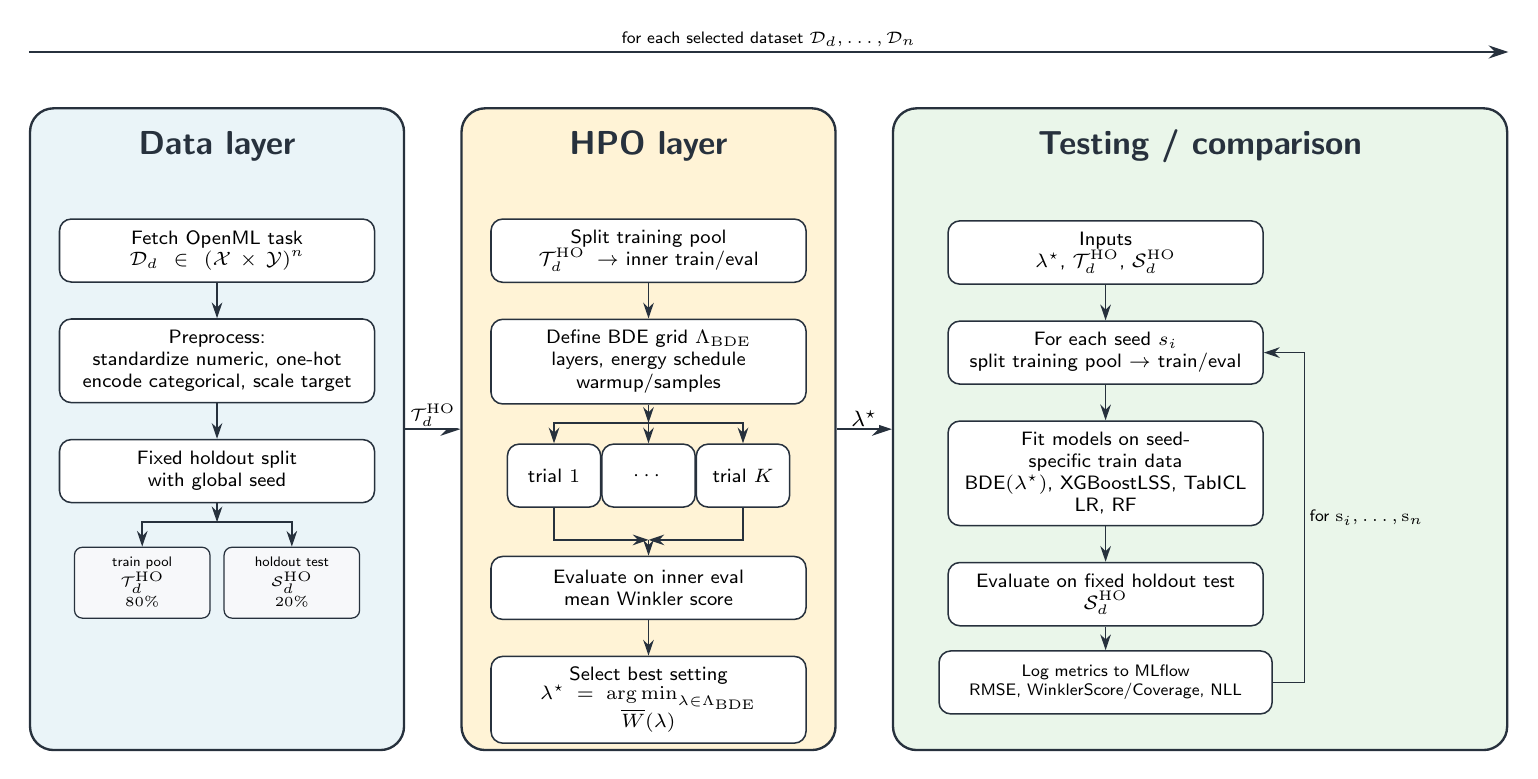
\begin{tikzpicture}[node distance=4.5mm and 7mm]

% ---------------------------------------------------------------------------
% Stage containers
% ---------------------------------------------------------------------------
\node[pipeline block=DataFill] (dataBlock) {};
\node[pipeline block=HpoFill, right=of dataBlock] (hpoBlock) {};
\node[pipeline block=TestFill, minimum width=7.8cm, right=of hpoBlock] (testBlock) {};

% Dataset-level loop: the complete workflow is repeated for every dataset.
\draw[main flow]
  ([yshift=7mm]dataBlock.north west) --
  node[above, dataset label] {for each selected dataset $\mathcal{D}_d,\ldots,\mathcal{D}_n$}
  ([yshift=7mm]testBlock.north east);

% ---------------------------------------------------------------------------
% Data layer: OpenML loading, preprocessing, and the fixed holdout split
% ---------------------------------------------------------------------------
\node[stage title] (dataTitle) at ([yshift=-5mm]dataBlock.north) {Data layer};

\node[pipeline step, below=6mm of dataTitle] (openml)
  {Fetch OpenML task\\[-0.2mm]$\mathcal{D}_d \in (\mathcal{X}\times\mathcal{Y})^n$};

\node[pipeline step, below=of openml] (preprocess)
  {Preprocess:\\standardize numeric, one-hot encode categorical, scale target};

\node[pipeline step, below=of preprocess] (holdout)
  {Fixed holdout split\\ with global seed};

\node[mini table, below=5.5mm of holdout, xshift=-9.5mm] (trainHO)
  {\begin{tabular}{@{}c@{}}
     train pool\\
     $\mathcal{T}^{\mathrm{HO}}_d$\\
     $80\%$
   \end{tabular}};

\node[mini table, below=5.5mm of holdout, xshift=9.5mm] (testHO)
  {\begin{tabular}{@{}c@{}}
     holdout test\\
     $\mathcal{S}^{\mathrm{HO}}_d$\\
     $20\%$
   \end{tabular}};

\coordinate[below=2.4mm of holdout] (holdoutFork);

\draw[flow] (openml) -- (preprocess);
\draw[flow] (preprocess) -- (holdout);
\draw[flow] (holdout) -- (holdoutFork);
\draw[flow] (holdoutFork) -| (trainHO.north);
\draw[flow] (holdoutFork) -| (testHO.north);

% ---------------------------------------------------------------------------
% HPO layer: train/eval split, BDE grid search, and best setting selection
% ---------------------------------------------------------------------------
\node[stage title] (hpoTitle) at ([yshift=-5mm]hpoBlock.north) {HPO layer};

\node[pipeline step, below=6mm of hpoTitle] (innerSplit)
  {Split training pool\\$\mathcal{T}^{\mathrm{HO}}_d \rightarrow$ inner train/eval};

\node[pipeline step, below=of innerSplit] (grid)
  {Define BDE grid $\Lambda_{\mathrm{BDE}}$\\layers, energy schedule\\warmup/samples};

% Repeated trial boxes visualize the Optuna grid search.
\foreach \x/\name/\body in {
  -12mm/trialA/{trial $1$},
  0mm/trialB/{$\cdots$},
  12mm/trialC/{trial $K$}
}{
  \node[compact step] (\name) at ([xshift=\x,yshift=-9mm]grid.south) {\body};
}

\begin{scope}[on background layer]
  \node[trial group, fit=(trialA)(trialB)(trialC)] (trialGroup) {};
\end{scope}

\node[pipeline step, below=4.5mm of trialGroup] (hpoScore)
  {Evaluate on inner eval\\mean Winkler score};

\node[pipeline step, below=of hpoScore] (bestLambda)
  {Select best setting\\[-0.4mm]
   $\lambda^\star=\operatorname*{arg\,min}_{\lambda\in\Lambda_{\mathrm{BDE}}}$\\[-0.4mm]
   $\overline{W}(\lambda)$};

\coordinate[below=2.3mm of grid] (trialFork);

\draw[flow] (innerSplit) -- (grid);
\draw[flow] (grid) -- (trialFork);
\foreach \name in {trialA,trialB,trialC}{
  \draw[flow] (trialFork) -| (\name.north);
}
\coordinate[above=2mm of hpoScore] (scoreFork);
\draw[flow] (trialA.south) |- (scoreFork);
\draw[flow] (trialC.south) |- (scoreFork);
\draw[flow] (scoreFork) -- (hpoScore.north);
\draw[flow] (hpoScore) -- (bestLambda);

% ---------------------------------------------------------------------------
% Testing and comparison: robust seed runs on the fixed holdout test set
% ---------------------------------------------------------------------------
\node[stage title] (testTitle) at ([yshift=-5mm]testBlock.north)
  {Testing / comparison};

\node[pipeline step, below=6mm of testTitle, xshift=-12mm] (testInput)
  {Inputs\\$\lambda^\star$, $\mathcal{T}^{\mathrm{HO}}_d$, $\mathcal{S}^{\mathrm{HO}}_d$};

\node[pipeline step, below=of testInput] (seedSplit)
  {For each seed $s_i$\\split training pool $\rightarrow$ train/eval};

\node[pipeline step, below=of seedSplit] (models)
  {Fit models on seed-specific train data\\BDE$(\lambda^\star)$, XGBoostLSS, TabICL\\LR, RF};

\node[pipeline step, below=of models] (evaluate)
  {Evaluate on fixed holdout test\\$\mathcal{S}^{\mathrm{HO}}_d$};

\node[pipeline step, below=3mm of evaluate, text width=3.95cm, font=\diagrammetricsfont] (metrics)
  {Log metrics to MLflow\\RMSE, WinklerScore/Coverage, NLL};

\draw[flow] (testInput) -- (seedSplit);
\draw[flow] (seedSplit) -- (models);
\draw[flow] (models) -- (evaluate);
\draw[flow] (evaluate) -- (metrics);

% Seed loop drawn inside the right side of the final block.
\coordinate (seedLoopA) at ([xshift=4mm]metrics.east);
\coordinate (seedLoopB) at ([xshift=4mm]seedSplit.east);
\draw[flow]
  (metrics.east) -- (seedLoopA) |- (seedLoopB) -- (seedSplit.east);
\coordinate (seedLoopMid) at ($(seedLoopA)!0.5!(seedLoopB)$);
\node[seed label, anchor=west] at ([xshift=1mm]seedLoopMid)
  {for $\mathrm{s}_i,\ldots,\mathrm{s}_n$};

% ---------------------------------------------------------------------------
% Cross-stage data flow
% ---------------------------------------------------------------------------
\draw[main flow]
  (dataBlock.east) --
  node[above, handoff label] {$\mathcal{T}^{\mathrm{HO}}_d$}
  (hpoBlock.west);

\draw[main flow]
  (hpoBlock.east) --
  node[above, lambda handoff label] {$\lambda^\star$}
  (testBlock.west);

\end{tikzpicture}
\end{document}
